\begin{figure*}[t]
\centering
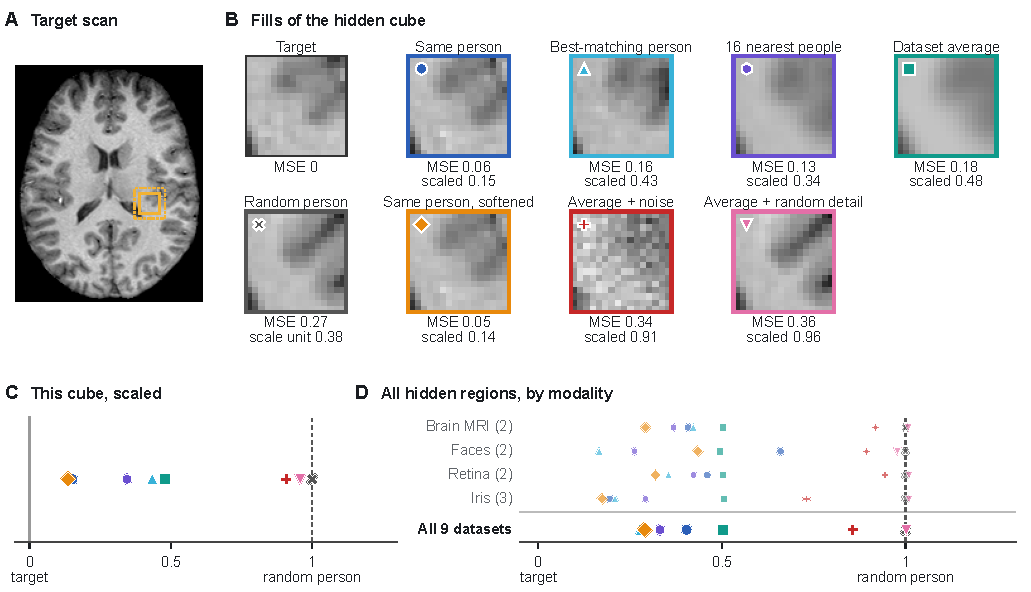
\includegraphics[width=0.86\textwidth]{fig/fig_explainer_mse_v3.pdf}
\caption{\textbf{How one row of Figure~\ref{fig:summary} is computed: \acs{MSE} on one brain cube.}
\textbf{A,} One QTIM brain scan; solid square: the hidden 16\,mm cube; dashed square: the 4\,mm ring of visible context around it.
\textbf{B,} The target cube and each fill, framed in its color and marker from Figure~\ref{fig:summary} (Section~\ref{sec:controls}): the same person's second scan; the best-matching person, the unrelated person whose cube is most like the target's (found by looking inside the hidden cube); the average of the 16 unrelated people with the most similar visible ring; the dataset average of all unrelated people; one random person; and three controls: the second scan with 85\% of its detail kept (softened), the average plus white noise, and the average plus a random person's detail, each at the same strength.
Below each fill: its \acs{MSE} to the target and that \acs{MSE} scaled by the average \acs{MSE} of 16 random people (0.38), so that 0 is the target and 1 is a random person.
\textbf{C,} The same cube on this scale.
\textbf{D,} Faint rows: means over all hidden regions and datasets of one modality (number of datasets in brackets); bold row: mean over the nine datasets, which is the \acs{MSE} row of Figure~\ref{fig:summary}.
PAPILA and IXI have no second image, so their same-person infill is the mirrored image of the other side.
The cube was chosen before drawing as the one of 1{,}472 complete cubes closest to the QTIM averages; brain values are provisional.
Even on one cube, \acs{MSE} scores the softened same person (0.14) as close as the same person (0.15) and puts the dataset average (0.48) at half a random person.}
\label{fig:explainer}
\end{figure*}
% Sources: make_fig_explainer_v3.py output (v1 figure kept as fig/fig_explainer_mse.pdf); results/donor_ladder_brain_metrics.json
% (lambda_shrink); results/cross_modality/common_all.json and fig_metric_summary_R.json (panel D).
